
\section{Arduino}
\label{sec:Arduino}
Der erste Arduino wurde 2005 von Hernando Barragan, Massimo Banzi und David Curatielles erfunden. Das Ziel war es einen Mikrocontroller-Board zu erfinden das sich einfach mit verschiedenen Dingen verbinden ließ und einfach zu Programmieren war. Da das Board von Studenten und Künstlern benutzt werden sollte stand auch der Preis des Boards im Vordergrund. Die Erfinder entschieden sich einen 8-bit Mikrocontroller der Atmel aus der AVR-Familie. Die Platine auf der der Mikrocontroller aufgebracht war erhielt einfache Ansteckmöglichkeiten, um etwa Sensoren, Relais und Motoren anschließen zu können. Die Erfinder schrieben zusätzlich einen Bootloader für den Mikrocontroller, der mit einfach mit der eigens entwickelten \ac{IDE} bespielt werden kann. Die Programmierung des Mikrocontrollers erfolgt mit C bzw. C++.

Über die Jahre wurden verschiedene Boards entwickelt die verschiedene Typen des Atmel Prozessoren nutzten. 2012 wurde sogar ein Arduino mit einem 32-Bit ARM Cortex-M3 Prozessor entwickelt. Die neueren Versionen der Arduino Boards haben bessere Prozessoren und mehr bzw. verbesserte Input / Output Pins Features. Die verschiedenen Boards unterscheiden sich hinsichtlich Größe, Form und zusätzliche Features wie zum Beispiel USB Anschluss und externer Stromversorgung.  Bei der Hardware, sowie der Software von Arduinos handelt es sich um ein Open-Source Projekt. Die Community von Arduino ist in den letzten Jahren ständig gewachsen, was zu einem die Fehlerbehandlung und die Suche nach neuen Ideen stark vereinfacht. Es gibt im Internet viele Do-It-Yourself Projekte, die die Nutzer mit detailreichen Anleitungen zum Ziel führen.

Trotz der vielen Möglichkeiten und der einfachen Programmierung mit Hilfe der Arduino IDE, dennoch gibt es einige kleine Einschränkungen die man bei Projekten beachten muss:
\begin{itemize}
	\item Der Speicher ist einer der größten Einschränkungen, da dieser meist nicht erweiterbar ist. Die verwendeten Mikrocontroller haben eine feste Größe für den Programm- und Variablenspeicher. Der Arduino war nie als Ersatz für ein komplettes Computersystem mit viel Arbeitsspeicher und einem großen dauerhaften Speichersystem gedacht.
	\item Die Geschwindigkeit des Arduinos ist eine weitere Einschränkung. Die typische Geschwindigkeit der CPU liegt zwischen 8 und 20 MHz. Dennoch ist diese Geschwindigkeit meist ausreichend. Da der Arduino meist nur eine dedizierte Aufgabe hat und diese relativ langsam geschehen. Zum Beispiel müssen die Sensorwerte bei einer Hausüberwachung nur jede Minute  ausgewertet werden. 
	\item Eine weitere Einschränkung ist der elektrische Strom. Da die Input / Output Pins direkt mit dem Mikrocontroller verbunden sind, ist Vorsicht geboten, welche Spannungen an diese angeschlossen werden. Sollte die Spannung zu hoch sein kann der Mikrocontroller zerstört werden. Die verschiedenen Mikrocontroller die in Arduinos verbaut sind arbeiten meist entweder mit 3,3 V oder mit 5 V. 
\end{itemize}
\subsection{AVR Microcontroller}
\label{sec:AvrMikrocontroller}
Der AVR Mikrocontroller wurde in den frühen 1990er als Studienprojekt und später von Atmel aufgekauft. Bei AVR Mikrocontroller handelt es sich um eine Harvard Architektur, bei der der Programmcode in einem Read-Only Speicher gespeichert wird und die modifizierbaren Variablen in einem separaten Speicherbaustein sind. Ein Mikrocontroller besteht dabei aus  einer AVR CPU und zusätzlich Peripherikomponenten wie Timers, Counters, Serielle Interface Logik, Analog Digital Wandler, Analog Comperators und diskrete digitale Input-Output Ports. 
\paragraph{Architektur}
Im Bild \ref{img:aufbauMikrocontroller} ist der der allgemeine Aufbau des AVR Mikrocontrollers zu sehen. Der Mikrocontroller besteht aus dem AVR Core, Speicherbausteinen (Flash Speicher und EEPROM und verschiedenen  pheripheralen Funktionen wie Input/Output, Analog-Digital Wandler, Zähler, Timer und ein Serielles Interface. Dabei sind in der folgende Liste die Grundspezifikationen des Mikrocontrollers zusammengefasst:
\begin{figure}
	\centering
	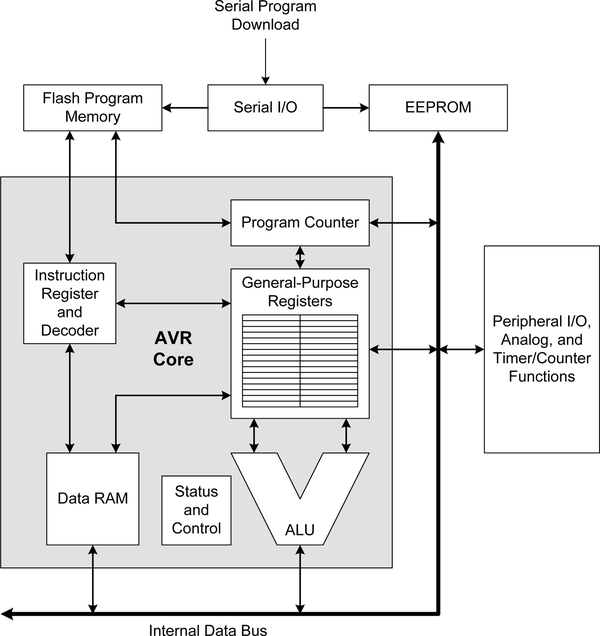
\includegraphics[width=0.9\textwidth]{bilder/aufbauMikrocontroller.png}
	\caption[Aufbau eines AVR Mikrocontrollers]{Aufbau eines AVR Mikrocontrollers. Quelle:\cite{hughes2016arduino}}
	\label{img:aufbauMikrocontroller}
\end{figure}
\begin{itemize}
\item RISC Architektur
\begin{itemize}
\item 131 Instruktionen
\item 32 8-bit General-Purpose-Register
\item Bis zu 20 MHz CPU Geschwindigkeit
\end{itemize}
\item Speicher
\begin{itemize}
\item Flash-Speicher (bis zu 256 Kilobytes)
\item EEPROM (bis zu 4 Kilobytes)
\item Interner SRAM (bis zu 32 Kilobytes)
\end{itemize}
\item Betriebsspannung
\begin{itemize}
\item Spannung zwischen 1,8 V und 5V
\end{itemize}
\end{itemize}
Der Mikrocontroller nutz drei verschiede Typen von Speicher, dem Flash Speicher, SRAM und dem EEPROM. Der Flash Speicher wird für die Speicherung des Programmcodes genutzt und ist nicht flüchtig. Beim SRAM handelt es sich um einen flüchtigen Speicher. Dieser speichert die Variablen des laufenden Programmes und enthält den Stack. Der EEPROM ist ein nicht flüchtiger Speicher, der Variablen dauerhaft speichern kann. Dieser speichert die Daten auch dann, wenn der Arduino keine Spannung anliegen hat. Der Nachteil eines EEPROMs ist jedoch die Zugriffsgeschwindigkeit im Gegensatz zum SRAM.
\paragraph{Peripherie}
Der folgende Abschnitt beschreibt die Peripherie des AVR-Mikrocontrollers, die an den internen Datenbus angeschlossen sind.
\paragraph{}
Innerhalb des Kontroll-Registers wird bestimmt wie die I/O Ports, der Timer, die Kommunikationsinterfaces und andere Funktionen funktionieren und reagieren. Das Kontroll-Register ist notwendig, da der AVR-Mikrocontroller deutlich mehr Funktionen hat wie Anschlüsse (Input/Output Pins). Zusätzlich können verschiedene Funktionen durch bestimmte Werte im Kontroll-Register verändert oder angepasst werden. Da das Kontroll-Register dynamisch konfigurierbar ist können Pins verschiedene Pins zu unterschiedlichen Zeiten und verschieden Funktionen haben. Ein Beispiel hierfür ist,  dass an einem Pin sowohl der Anlog Vergleicher angeschlossen ist und der Pin als Interrupt Quelle genutzt werden kann.
\paragraph{}
Der AVR-Mikrocontroller besitzt mehrere digitale Input/Output Ports um mit der externen Umgebung zu kommunizieren. Die Ports sind bidirektional, was bedeutet,  dass sie sowohl als Input als auch als Output genutzt werden können. Jeder Pin besitzt eine interne Logik die festlegt ob es sich um einen Input oder Output handelt und ob ein Pull-Up Widerstand benutzt wird. Die interne Logik verfügt über viele Funktionen, die Einzel konfiguriert werden können.
\paragraph{}
In einem AVR-Mikrocontroller ist sowohl ein 8-Bit als auch ein 16-Bit Timer/Counter verbaut. Es kann zwischen zwei Modis unterschieden werden. Zu einem das Hochzählen mit Hilfe des internen Taktes und zum anderen mit Hilfe  einer externen Quelle. Bei einem Überlaufen(Overflow) des Registers wird das Register wieder auf Null gesetzt, da das Register nur eine bestimmte Speicherbreite hat (8 bzw. 16 Bit). Bei einem Überlauf besteht die Möglichkeit einen Interrupt auszulösen.
\paragraph{}
Mit Hilfe des Prescalers können die Zählraten des Timers bzw. des Counters angepasst werden. Der Prescaler nutzt die interne Uhr der CPU um nach einem bestimmten Wert diese zu dividieren. Dies bedeutet, dass der Timer/Counter nur nach jedem X. Takt hochgezählt wird. Als Divisor zur Verlangsamung steht 8, 64, 256 oder 1024 zur Verfügung. So kann der Timer/Counter besser an die reale Umgebung angepasst werden, da wiederkehrende Events meist erst nach Sekunden  und nicht nach Mikrosekunden passieren sollen. 
\paragraph{}
Fast alle AVR-Mikrocontroller haben direkt einen Analog Komperator integriert. Der Komperator hat zwei Eingänge, einen nomalen und einen invertierten. Der Analog Komperator vergleicht nun beide Spannungen miteinander und gibt aus welche der beiden Spannungen größer ist.
\paragraph{}
Mit Hilfe eines Analog zu Digital Wandler können sehr einfach analoge Größen in einen Digitalen Wert gewandelt werden. Ein Analog-Digital Wandler besitz meist zwischen 4 und 28 Inputs (sogenannte Kanäle).Da der Mikrocontroller nur einen Analog-Digital Wandler ist oder hat, besitzt dieser zusätzlich einen Multiplexer, der die verschiedenen Kanäle auf den Analog-Digital Wandler schaltet. Für eine Umwandlung werden ca. 65 Mikrosekunden benötigt.
\paragraph{}
Der AVR-Mikrocontroller bietet drei verschiedene Formen eines seriellen Interfaces: 
\begin{itemize}
\item \ac{USART} : Diese Schnittstelle erlaubt eine synchrone oder asynchrone serielle Datenübertragung. Die häufigsten Anwendungsgebiete sind die Kommunikation mit dem PC, Datenübertragung mit einer IR oder einem Bootloader.
\item \ac{SPI} (siehe Kapitel \ref{sec:I2C})
\item Two-Wire Interface: Diese Schnittstelle ist kompatible  mit dem $I^{2}C$ Protokoll(siehe Kapitel \ref{sec:I2C} )
\end{itemize}
\paragraph{Interrupts}
Bei einem Interrupt handelt es sich um eine Unterbrechungsanforderung des normalen Programmablaufs. Ein Interrupt kann durch verschiedene Szenarien ausgelöst werden:
\begin{itemize}
\item Interrupt durch einen externen Pin
\item Interrupt durch den Timer/Counter
\item Interrupt durch die Fertigstellung einer Seriellen Übertragung
\item Interrupt wenn der EEPROM mit dem Speichern bzw. Lesen von Daten fertig ist
\end{itemize}
Wenn ein Interrupt detektiert wurde wird das gerade ausgeführte Programm unterbrochen und die sogrannte Interrupt Service Routine aufgerufen. Wenn diese fertig ausgeführt wurden wird das Programm an der unterbrochenen Stelle wieder ausgeführt. 
Die Interrupts können im Kontroll-Register zu einem zum Global aktiviert werden und zum anderen können einzelne Interrupts an und ausgeschalten werde. Wenn ein Interrupt passiert wird in der Interrupt Vektor Tabelle nachgeschaut an welcher Stelle sich die Interrupt Service Routine befindet.
\paragraph{Watchdog Timer}
Der AVR-Mikrocontroller besitzt einen Watchdog Timer (\ac{WDT}). Der WDT besitzt eine einstellbare Zeit zwischen 16 ms und 8s. Wenn es beim WDT zu einem Overflow kommt wird entweder der Programmcounter auf 0 zurückgesetzt (Reset-Modus) , ein Interrupt generiert oder eine Kombination aus beidem. Da der Watchdog Timer einen seperaten Oszillator besitzt, wird der  WDT auch im Sleep Modus weiter hochgezählt. Dies kann genutzt werden um den Mikrocontroller nach einer bestimmten Zeit wieder zu aktivieren. Sollte der WDT im Reset Modus sein, so können damit Deadlocks verhindert werden, wenn zum Beispiel der WDT nicht mehr Softwareseitig zurückgesetzt wird.

\subsection{Arduino Nano /  Pro Mini}
In dieser Studienarbeit werden zwei unterschiedliche Arduino Boards eingesetzt, weshalb der Arduino Nano und Arduino Pro Mini in diesem Abschnitt genauer betrachtet wird.

In beiden Arduinos ist der ATmega328 verbaut. Dieser ist aus der Produktfamilie der AVR-Mikrocontroller. Im Folgenden werden die gemeinsamen Eigenschaften der Arduinos aufgelistet: 
\begin{itemize}
	\item Speicherkapazität
\begin{itemize}
	\item Programmspeicher/Flash Speicher: 32 Kilobytes
	\item EEPROM 1 Kilobytes
	\item SRAM 2 Kilobytes
\end{itemize}
	\item Taktfrequenz: 16 MHz
	\item Externe Interrupts: 2
	\item Analoge I/O Pins: 8
	\item Digitale I/O Pins: 14
	\item Betriebsspannung: 5 V
\item Versorgungsspannung: 5V – 12V
\end{itemize}
Die beiden Boards unterscheiden sich vor allem in der Größe und zusätzlichen Ausstattung.  Der Arduino Nano hat eine Größe von $18$ x $45 mm$, wohingegen der Arduino Pro Mini nur eine Größe von $18$ x $33 mm$ besitzt.

Hinsichtlich der Ausstattung unterscheiden sich die zwei Modell  sehr deutlich. Der Arduino Nano besitzt einen Mini USB Anschluss.  Dieser kann zu einem zur Stromversorgung genutzt werden, zum anderen kann der Arduino Nano über den USB Anschluss programmiert werden. Der Arduino Pro Mini hingegen hat keine USB Anschluss. Um den Pro Mini zu programmieren wird ein USB-RS232-Interface-Chips benötigt. Mit diesem ist es möglich eine serielle Schnittstelle über USB verfügbar zu machen. Eines der bekanntesten Programmern  ist von der schottischen Firma Future Technology Devices International (FTDI). Der Arduino Nano besitzt im Gegensatz zum Pro Mini bereits auf dem Board einen 5V zu 3,3 V Wandler. Zusammenfassend kann gesagt werden, dass der Arduino Pro Mini eine reduzierte Version des Arduino Nano’s ist.  


\subsection{Software}
Dieses Unterkapitel betrachtet die Softwareumgebung, sowie die genutzte Entwicklungsumgebung auf dem Arduino.
\paragraph{C/C++} Das Arduino Board kann mit Hilfe von C oder C++ oder mit einer reduzierten Version von C, der sogenanten „Arduin Programming Language“, programmiert werden. Diese enthält die Grundoperatoren, Variablen und Funktionen.  Zur Kompilation des  Programmcodes wird  der GNU avr-gcc Compiler verwendet. 

C und C++ werden vor allem für eine effiziente und maschinennahe Programmierung eingesetzt.  C++, sowie C bestehen nur aus sehr wenigen Schlüsselwörtern. Sie können jedoch mit Bibliotheken erweitert werden. Bei C++ handelt es sich um eine Erweiterung von dem C Standard von 1990. C++ bietet gegenüber von C mehr Datentypen, Ausnahmebehandlung, das Überladen von Operationen und weitere Funktionen, wie zum Beispiel virtuelle Funktionen. 

\paragraph{Arduino IDE} Die ebenfalls von Arduino erhältliche IDE ermöglicht das einfache Schreiben von Code und das Uploaden auf die Arduino Boars. Die Arduino IDE ist Open-Source und für Windows Mac OS X und für Linux erhältlich. Während der Studienarbeit wurde die Version 1.8.2 eingesetzt. Die Entwicklungsumgebung bietet dabei viele Features.
\begin{figure}
	\centering
	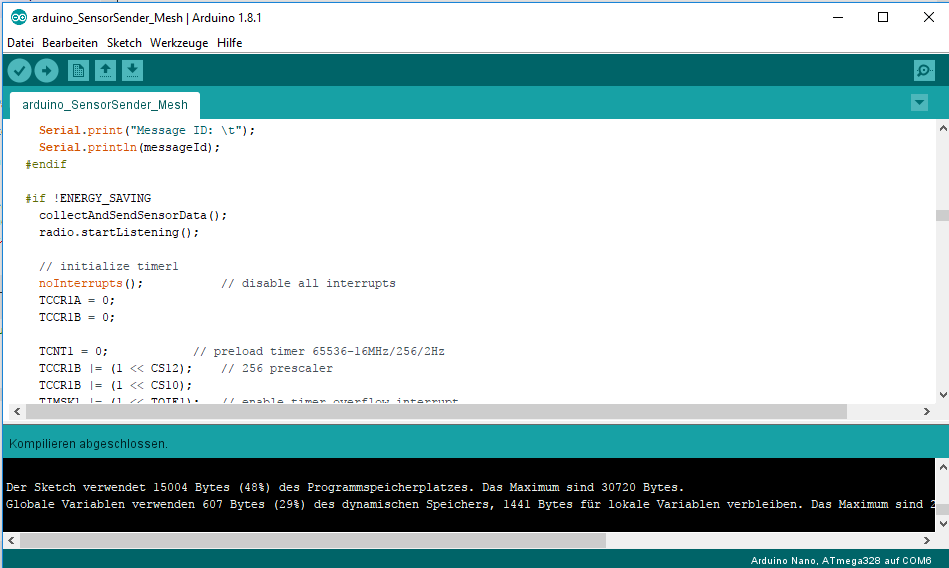
\includegraphics[width=0.9\textwidth]{bilder/arduinoIDE}
	\caption{Arduino IDE  1.8.1}
	\label{img:ArduinoIDE}
\end{figure}

\begin{itemize}
\item Kompilieren und Hochladen des Programmcodes auf den Arduino
\item Einbinden von externen Bibliotheken
\item Übersichtliches Bedienkonzept
\item Serieller Monitor zur Ausgabe von Daten des Arduinos
\end{itemize}
Die Arduino IDE zeichnet sich vor allem durch seine Einfachheit aus. Dies ermöglicht einen schnellen Einstieg in die Programmierung des Arduinos(siehe Grafik \ref{img:ArduinoIDE}).
